\documentclass[../main]{subfiles}

\begin{document}
\chapter{Electromagnetismo}
\info{
Contenido}{
Campo magnético creado por una corriente eléctrica, intensidad de campo, 
inducción, permeabilidad magnética, fuerza magnetomotriz, electroimanes.
}
\actividad{Resolver los siguientes problemas}
\begin{enumerate}
    
\item Se está fabricando un brazo robot que necesita levantar una lata de 
  conservas de durazno al natural que está hecha de hojalata recubierta 
  por una capa de estaño despreciable (equivalente a chapa normal), 
  para esto el equipo de producción pensó en diferentes alternativas, 
  una de ellas es fabricar un electroimán, para ello se hizo un electroimán 
  con núcleo de chapa silicio con las siguientes características: $N=150$, $i=0.4A$,$S=3cm^2$,$L=3cm$ ¿Podrá levantar la lata?
    \item Determinar la fuerza con la que atraerá un electroimán de armadura de hierro si la inducción que aparece en el núcleo es de $1,3T$ y la superficie de total de contacto entre el núcleo y el hierro móvil es de $4cm^2$ 
    \item Se desea conseguir que el electroimán de un contacto automático desarrolle una fuerza de atracción al bloque de contactos móviles de $2Kg$. Teniendo en cuenta que el núcleo está fabricado de hierro forjado, que posee 2000 espiras y que las dimensiones y forma del circuito magnético de dicho electroimán son las que se muestran en la siguiente figura, calcular la intensidad de la corriente eléctrica para conseguirlo.
    \begin{center}
    
\includegraphics[]{images/01/herradura.png}
    \end{center}
    \item Calcular la permeabilidad absoluta para una lámina de hierro que si es afectada por una intensidad de campo de 400Av/m adquiere una inducción magnética $B=1Tesla$.
    \item Si  $\mu_r=\mu/\mu_o$ y $\mu_o= 4\pi10^{-7}H/m$. Calcular la permeabilidad relativa $\mu_r$ para el problema anterior.
    \item Una chapa de silicio es sometida a un campo magnético de 9000Av/m según el cuadro 1 determinar la inducción $B$ en Teslas.
    \item Usando el cuadro 1 determinar la permeabilidad absoluta $\mu$ para Chapa normal con intensidades de campo de $H=100Av/m$, $H=1200Av/m$, $H=10000Av/m$
    \item Usando el cuadro 1 determinar la permeabilidad relativa $\mu_r$ para hierro forjado expuesto a intensidad de campo $H=120$, $H=2400$, $H=27000$ y $H=580$.
    \item Completar la siguiente tabla completando las permeabilidades relativas y absolutas  ¿La permeabilidad varía?
   
   \ejemplo{
   Ejemplo}{
   
   Calculamos la permeabilidad absoluta $\mu$ y la relativa $\mu_r$ 
   \begin{equation}
       \mu = B/H =0.1/80 = 0.00125
   \end{equation}
   \begin{equation}
       \mu_o = 4\pi x10^{-7}
   \end{equation}
    \begin{equation}
       \mu_r = \mu/\mu_o=\mu/(4\pi x10^{-7}) =0.00125/(4\pi x10^{-7}) = 994.72
   \end{equation}
  
   }
   
    \begin{table}[ht]
\begin{center}
\footnotesize	
\begin{tabular}[c]{|l|l|l|l|p{1cm}|p{1cm}|p{1cm}|p{1cm}|p{1cm}|p{1cm}|}
 \hline
  & \multicolumn{3}{|c|}{$H(Av/m)$} &\multicolumn{3}{|c|}{$\mu (Per.abs.)$} &\multicolumn{3}{|c|}{$\mu_r (Per.rel.)$}  \\
 \hline
 {$B(Teslas)$} &H.Forj.& CH.Nor. & H.Sil.&H.Forj.& CH.Nor. & H.Sil.&H.Forj.& CH.Nor. & H.Sil.  \\
 \hline
 0,1 & 80 & 50 & 90 &0.00125 & & &994.72 & & \\ \hline
 0,3 & 120 & 65&140 &0.0025 & & &1989.43 & &\\\hline
 0,5&160&100&170& & & & & &\\\hline
 0,7&230&180&240& & & & & &\\\hline
 0,9&400&360&350& & & & & &\\\hline
 1,1&650&675&530& & & & & &\\\hline
 1,3&1000&1200&1300& & & & & &\\\hline
 1,5&2400&2200&5000& & & & & &\\\hline
 1,6&5800&3500&9000& & & & & &\\\hline
 1,7&7000&5000&16500& & & & & &\\\hline
 1,8&11000&10000&27500& & & & & &\\\hline
 1,9&17000&16000& & & & & & &\\\hline
 2&27000&32000& & & & & & &\\ \hline
\end{tabular}
\end{center}
\end{table}
\newpage
    \item Construya 2 gráficos chapa normal y chapa silicio. Donde el eje x sea la la intensidad de campo $H[Av/m]$ y el eje Y sea la inducción magnética $B[Teslas]$
    Ejemplo para Hierro Forjado:
    \begin{table}[ht]
        \centering
        \begin{tabular}{c|c}
            x:$H[Av/m]$ & y:$B[Teslas]$ \\ \hline
             80&0,1 \\ 
            120 &0,3 \\
            160 &0,5 \\
            230 &0,7 \\
            400 &0,9 \\
            650 &1,1  \\
1000 & 1,3 \\
2400 &1,5 \\
5800 &1,6 \\
7000 &1,7 \\
11000 &1,8 \\
17000 &1,9 \\
27000 &2\\
    \end{tabular}
    \caption{Tabla para Hierro Forjado}
    \end{table}

\begin{center}
    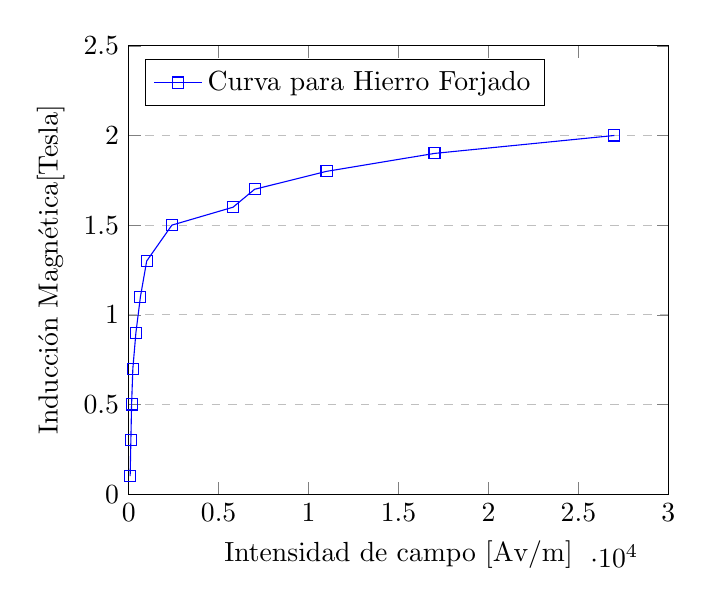
\begin{tikzpicture}
    
\begin{axis}[
    xlabel={Intensidad de campo [Av/m]},
    ylabel={Inducción Magnética[Tesla]},
    xmin=0, xmax=30000,
    ymin=0, ymax=2.5,
    xtick={0,5000,10000,15000,20000,25000,30000},
    ytick={0,0.5,1,1.5,2,2.5},
    ymajorgrids=true,
    legend pos=north west,
    grid style=dashed,
]

\addplot[
    color=blue,
    mark=square,
    ]
    coordinates {
     (80,0.1)( 120,0.3 )( 160,0.5 )( 230,0.7 )( 400,0.9 )( 650,1.1 )(1000,1.3)(2400,1.5)(5800,1.6)(7000,1.7 )(11000,1.8 )(17000,1.9)(27000,2.)};
\legend{Curva para Hierro Forjado};
\end{axis}

\end{tikzpicture}

    \end{center}
\end{enumerate}    
\end{document}
